%#%#%#%#%#%#%#%#%#%#%#%#%#%#%#%#%#%#%#%#%#%#%#%#%#%#%#%#%#%#%#%#%#%#%#
% chapter-1.tex
%#%#%#%#%#%#%#%#%#%#%#%#%#%#%#%#%#%#%#%#%#%#%#%#%#%#%#%#%#%#%#%#%#%#%#

% Source: TAoMP, Chapter 1 — "Introduction"

%%%%%%%%%%%%%%%%%%%%%%%%%%%%%%%%%%%%%%%%%%%%%%%%%%%%%%%%%%%%%%%%%%%%%%%%%%%%%%%%%%%%%%%%
\examnewsection[TAoMP, Chapter 1 — Introduction]
%%%%%%%%%%%%%%%%%%%%%%%%%%%%%%%%%%%%%%%%%%%%%%%%%%%%%%%%%%%%%%%%%%%%%%%%%%%%%%%%%%%%%%%%

% Lorem ipsum dolor sit amet, consectetur adipisicing elit, sed do eiusmod tempor incididunt ut labore et dolore magna aliqua. Ut enim ad minim veniam, quis nostrud exercitation ullamco laboris nisi ut aliquip ex ea commodo consequat. Duis aute irure dolor in reprehenderit in voluptate velit esse cillum dolore eu fugiat nulla pariatur. Excepteur sint occaecat cupidatat non proident, sunt in culpa qui officia deserunt mollit anim id est laborum.


% An example of a simple/plain question
\question 
\Bloom{REMEMBER} % <=== Bloom level (shown only with answers)
Lorem ipsum dolor sit amet, consectetur adipisicing elit, sed do eiusmod tempor incididunt?
\begin{choices}
\CHOICE Lorem ipsum dolor sit amet, consectetur adipisicing elit, sed do eiusmod tempor incididunt ut labore et dolore magna aliqua.
\choice Ut enim ad minim veniam, quis nostrud exercitation ullamco laboris nisi ut aliquip ex ea commodo consequat.
\choice Duis aute irure dolor in reprehenderit in voluptate velit esse cillum dolore eu fugiat nulla pariatur.
\choice Excepteur sint occaecat cupidatat non proident, sunt in culpa qui officia deserunt mollit anim id est laborum.
\end{choices}



% An example of a simple/plain question, with multiple answers in the same line
% Using the exam standard 'parchoices' enviornment
\question 
\Bloom{REMEMBER}
Lorem ipsum dolor sit amet, consectetur adipisicing elit $(N \ge 3)$?
\\
\begin{oneparchoices}
\choice Smal.
\choice $N$
\CHOICE A very long choice.
\choice Quite exactly $N$.
\end{oneparchoices}



% An example of a simple/plain question, with multiple answers in the same line
% Use the optional 'choices' argument, e.g., [4], to put the answers in multiple
% columns, instead of one answer per line
\question 
\Bloom{REMEMBER}
Lorem ipsum dolor sit amet, consectetur adipisicing elit $(N \ge 3)$?
\begin{choices}[4]  % <=== The number of columns for the maswers
\choice Smal.
\choice $N$
\CHOICE A very long choice.
\choice Quite exactly $N$.
\end{choices}



% Another example with multiple (two) answers per line
\question 
\Bloom{REMEMBER}
Duis aute irure dolor in reprehenderit in voluptate velit esse cillum dolore eu fugiat nulla pariatur?
\begin{choices}[2]
\CHOICE \texttt{while}, \texttt{for}, and \texttt{repeat}.
\choice \texttt{while}, \texttt{foreach}, and \texttt{repeat}.
\choice \texttt{continue}, \texttt{if-then-else}, and \texttt{for}.
\choice \texttt{stop}, \texttt{continue}, and \texttt{if-then-else}.
\end{choices}



% An example with a LARGE code on the right
% Splits the text width into 65% on the left, for the question and answers, 
% and 35% on the right, for the code block
\question 
\begin{splitquestion}{0.35} % <=== right side is 35% of text width
% Left side starts here
\Bloom{EVALUATE}
Excepteur sint occaecat cupidatat non proident, sunt in culpa qui officia deserunt mollit anim id est laborum?
\begin{choices}[4]
\choice 15
\CHOICE 14
\choice 11
\choice 10
\end{choices}
% Left side ends here
\nextpart % <=== right side is 35% of text width
% Right side starts here
\begin{java}
Counter counter = new Counter(1);
void primePrint() {
  long i = 0;
  long limit = 10;
  while (i < limit) {
    i = counter.getAndIncrement();
    print(i);
  }
}  
\end{java}
% Right side ends here
\end{splitquestion}



% \clearpage % <==== use '\clearpage' to force a page break



% An example with a SMALL code on the right
% Splits the text width into 65% on the left, just for the question, 
% and 35% on the right, for the code block
% the questions are below and use 100%
\question 
\begin{splitquestion}{0.32}
\Bloom{UNDERSTAND}
Lorem ipsum dolor sit amet, consectetur adipisicing elit, sed do eiusmod tempor incididunt ut labore et dolore magna aliqua. Ut enim ad minim veniam, quis nostrud exercitation ullamco laboris nisi ut aliquip ex ea commodo consequat?
\nextpart
\begin{java}
public interface Consensus<T> {
    T decide(T value);
}
\end{java}
\end{splitquestion}
\begin{choices} % <=== Questions are after the '\end{splitquestion}', so use 100%
\choice Lorem ipsum dolor sit amet, consectetur adipisicing elit, sed do eiusmod tempor incididunt ut labore et dolore magna aliqua.
\CHOICE Ut enim ad minim veniam, quis nostrud exercitation ullamco laboris nisi ut aliquip ex ea commodo consequat.
\choice Duis aute irure dolor in reprehenderit in voluptate velit esse cillum dolore eu fugiat nulla pariatur.
\choice Excepteur sint occaecat cupidatat non proident, sunt in culpa qui officia deserunt mollit anim id est laborum.
\end{choices}



% An example of a question with pieces of code in the answers
\question
\Bloom{CREATE}
Lorem ipsum dolor sit \(r\) consectetur \(v_0\).  Ut enim ad minim veniam, quis nostrud exercitation ullamco laboris nisi ut aliquip ex ea commodo consequat?
\begin{choices}[2]
\choice 
\begin{java}[bgcolor=white,samepage]
propose(value);
if (r.get() == §$v_0$§) {
  r.getAndSet(myId);
  decide(my value);
} else decide(other value);
\end{java}
\choice 
\begin{java}[bgcolor=white,samepage]
propose(value);
r.getAndSet(myId);
decide(my value);
§~§
§~§
\end{java}
\CHOICE 
\begin{java}[bgcolor=white,samepage]
propose(value);
old = r.getAndSet(myId);
if (old == §$v_0$§) decide(my value);
else decide(other value);
§~§
\end{java}
\choice 
\begin{java}[bgcolor=white,samepage]
propose(value);
while (r.get() != myId) {}
r.getAndSet(myId); 
decide(my value);
§~§
\end{java}
\end{choices}



% An example with LOTS of code
% The code is below the question (before the answes) and not on the side
\question 
\Bloom{CREATE}
Lorem ipsum dolor sit amet, consectetur adipisicing elit, sed do eiusmod tempor incididunt ut labore et dolore magna aliqua. Ut enim ad minim veniam, quis nostrud exercitation ullamco laboris nisi ut aliquip ex ea commodo consequat?
\begin{multicols}{2}
\begin{minipage}{\linewidth}
\begin{java}
class Bakery implements Lock {
  private final boolean[] flag;
  private final int[] label;
  public Bakery(int n) {
    flag = new boolean[n];
    label = new int[n];
    for (int i = 0; i < n; i++) {
      flag[i] = false;
      label[i] = 0;
    }
  }
\end{java}
\end{minipage}
\begin{minipage}{\linewidth}
\begin{java}
  private int maxLabel() {
    int m = 0;
    for (int x : label) {
      if (x > m) m = x;
    }
    return m;
  }
\end{java}
\end{minipage}
\begin{minipage}{\linewidth}
\begin{java}
  public void lock() {
    int i = ThreadID.get();
    flag[i] = true;
    label[i] = maxLabel() + 1;
    for (int k = 0; k < label.length; k++) {
      if (k == i) continue;
      while (flag[k] && (label[k] < label[i] 
          || (label[k] == label[i] && k < i))) {
        // wait
      }
    }
  }
\end{java}
\end{minipage}
\begin{minipage}{\linewidth}
\begin{java}
  public void unlock() {
    int i = ThreadID.get();
    flag[i] = false;
  }
}  
\end{java}
\end{minipage}
\end{multicols}
\begin{choices}
\choice Lorem ipsum dolor sit amet, consectetur adipisicing elit, sed do eiusmod tempor incididunt ut labore et dolore magna aliqua.
\choice Ut enim ad minim veniam, quis nostrud exercitation ullamco laboris nisi ut aliquip ex ea commodo consequat.
\choice Duis aute irure dolor in reprehenderit in voluptate velit esse cillum dolore eu fugiat nulla pariatur.
\CHOICE Excepteur sint occaecat cupidatat non proident, sunt in culpa qui officia deserunt mollit anim id est laborum.
\end{choices}



% An example with an image on the side of the answers
% Question use 100%
% Answers use 50%
% Image uses 50%
\question 
\Bloom{UNDERSTAND}
Excepteur sint occaecat cupidatat non proident, sunt in culpa qui officia deserunt mollit anim id est laborum?
\begin{splitquestion}{0.5}
\begin{choices}
\choice Lorem ipsum dolor sit amet, consectetur adipisicing elit, sed do eiusmod tempor incididunt ut labore et dolore magna aliqua.
\CHOICE Ut enim ad minim veniam, quis nostrud exercitation ullamco laboris nisi ut aliquip ex ea commodo consequat.
\choice Duis aute irure dolor in reprehenderit in voluptate velit esse cillum dolore eu fugiat nulla pariatur.
\choice Excepteur sint occaecat cupidatat non proident, sunt in culpa qui officia deserunt mollit anim id est laborum.
\end{choices}
\nextpart
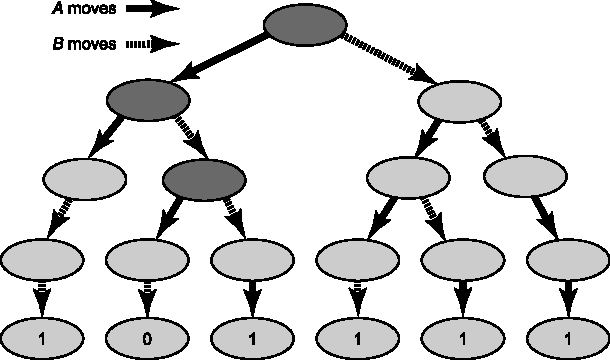
\includegraphics[width=\linewidth,align=t]{ch05 - TAoMP - fig_5.2}
\end{splitquestion}



% 2: Monte Carlo Method for $\pi$
\question
\begin{splitquestion}{0.1}
\Bloom{REMEMBER}
Lorem ipsum dolor sit amet, consectetur adipisicing elit, sed do eiusmod tempor incididunt ut labore et dolore magna aliqua. Ut enim ad minim veniam, quis nostrud exercitation ullamco laboris nisi ut aliquip ex ea commodo consequat \(r = 1\) (see illustrative figure on the right)?
\nextpart
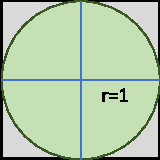
\includegraphics[width=\linewidth,align=t]{P01 Monte Carlo PI Java - fig1}
\end{splitquestion}
\begin{choices}[4]
\choice \(\rho = \pi^2\)
\CHOICE \(\rho = \frac{\pi}{4}\)
\choice \(\rho = \frac{1}{\pi}\)
\choice \(\rho = \frac{4}{\pi}\)
\end{choices}


